\part{Beschreibung des Projekts}
Der vorliegende Programmentwurf beschäftigt sich mit der
Visualisierung von Wegfinde-Algo\-rithmen.
Die Verfahren werden auf einem Gitter durchgeführt und
verfolgen hierbei das Ziel, den kürzesten Weg zwischen zwei Punkten
\texttt{S} und \texttt{Z} zu finden.
Die grundlegende Idee dieser Darstellungsmethode ist in
\autoref{fig-pathfinding-example} zu sehen.
Die gelb markieren Koordinaten zeigen den kürzesten Weg und die
grau eingefärbten Felder stellen Hindernisse dar.

\begin{figure}[h!]
  \center
  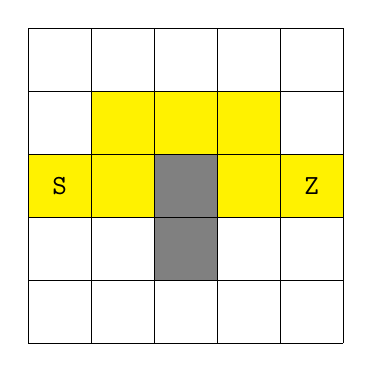
\begin{tikzpicture}
    [
      scale=0.8,
      every node/.style={black},
      path/.style={fill=yellow},
      wall/.style={fill=gray},
    ]

    \draw[step=1cm] (0,0) grid (5,5);

    \draw [wall] (2,2) rectangle (3,3);
    \draw [wall] (2,1) rectangle (3,2);
    
    \draw [path] (0,2) rectangle (1,3) node [midway, font=\ttfamily] {S};
    \draw [path] (1,2) rectangle (2,3);
    \draw [path] (1,3) rectangle (2,4);
    \draw [path] (2,3) rectangle (3,4);
    \draw [path] (3,3) rectangle (4,4);
    \draw [path] (3,2) rectangle (4,3);
    \draw [path] (4,2) rectangle (5,3) node [midway, font=\ttfamily] {Z};
  \end{tikzpicture}
  \caption{Wegfinde-Algorithmus}
  \label{fig-pathfinding-example}
\end{figure}

\noindent
Es wird unterschieden zwischen gewichteten und ungewichteten
Algorithmen. Ein gewichtetes Verfahren kann während der Wegsuche zusätzlich
Streckenkosten beachten (z.\,B. bei einem Stau)
und somit nicht nur den kürzesten, sondern
auch den günstigsten Weg finden. Kosten/Gewichte können auf dem Gitter durch
Zahlen dargestellt werden, wie in \autoref{fig-pathfinding-example-weight}
zu sehen ist.

\begin{figure}[h!]
  \center
  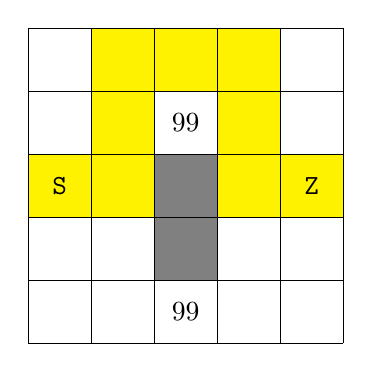
\begin{tikzpicture}
    [
      scale=0.8,
      every node/.style={black},
      path/.style={fill=yellow},
      wall/.style={fill=gray},
    ]

    \draw[step=1cm] (0,0) grid (5,5);

    \draw [wall] (2,2) rectangle (3,3);
    \draw [wall] (2,1) rectangle (3,2);
    
    \draw [path] (0,2) rectangle (1,3) node [midway, font=\ttfamily] {S};
    \draw [path] (1,2) rectangle (2,3);
    \draw [path] (1,3) rectangle (2,4);
    \draw [path] (1,4) rectangle (2,5);
    \draw [path] (2,4) rectangle (3,5);
    \draw [path] (3,4) rectangle (4,5);
    \draw [path] (3,3) rectangle (4,4);
    \draw [path] (3,2) rectangle (4,3);
    \draw [path] (4,2) rectangle (5,3) node [midway, font=\ttfamily] {Z};

    \draw (2,0) rectangle (3,1) node [midway] {99};
    \draw (2,3) rectangle (3,4) node [midway] {99};
  \end{tikzpicture}
  \caption{Wegfinde-Algorithmus mit Gewicht}
  \label{fig-pathfinding-example-weight}
\end{figure}

\noindent
Das Projekt besteht aus zwei Teilen: Der API
(ASP.NET Core Web API, im Ordner \enquote{\texttt{api}}) und der Benutzeroberfläche
(Vue, im Ordner \enquote{\texttt{vue}}). Der Quelltext
ist über den folgenden Link auf GitHub zu finden.
\footnote{\url{https://github.com/JensDll/pathfinding-visualization}}